% !TEX root = ../main.tex
% --+ 10.41 RG-F Experiment +---------------------------------------------------
\begin{frame}{Run Group F (RG-F) Experiment}
    \label{10.41::rgf_experiment}

    \begin{itemize}
        \item
            The RG-F experiment ran at Hall B during \ef{Spring} and \ef{Summer 2020}.

        \item
            Its target is composed of a D2 gas at room temperature.

        \item
            The RG-F target is 55 cm long in $z$, \ef{allowing us to compare acceptance across the scattering chamber}.
    \end{itemize}

    % TODO. Figure pending until CCTVal fixes connection to JLab.
    % \begin{center}
    %     \begin{figure}[t]
    %         \centering{
    %             \fbox{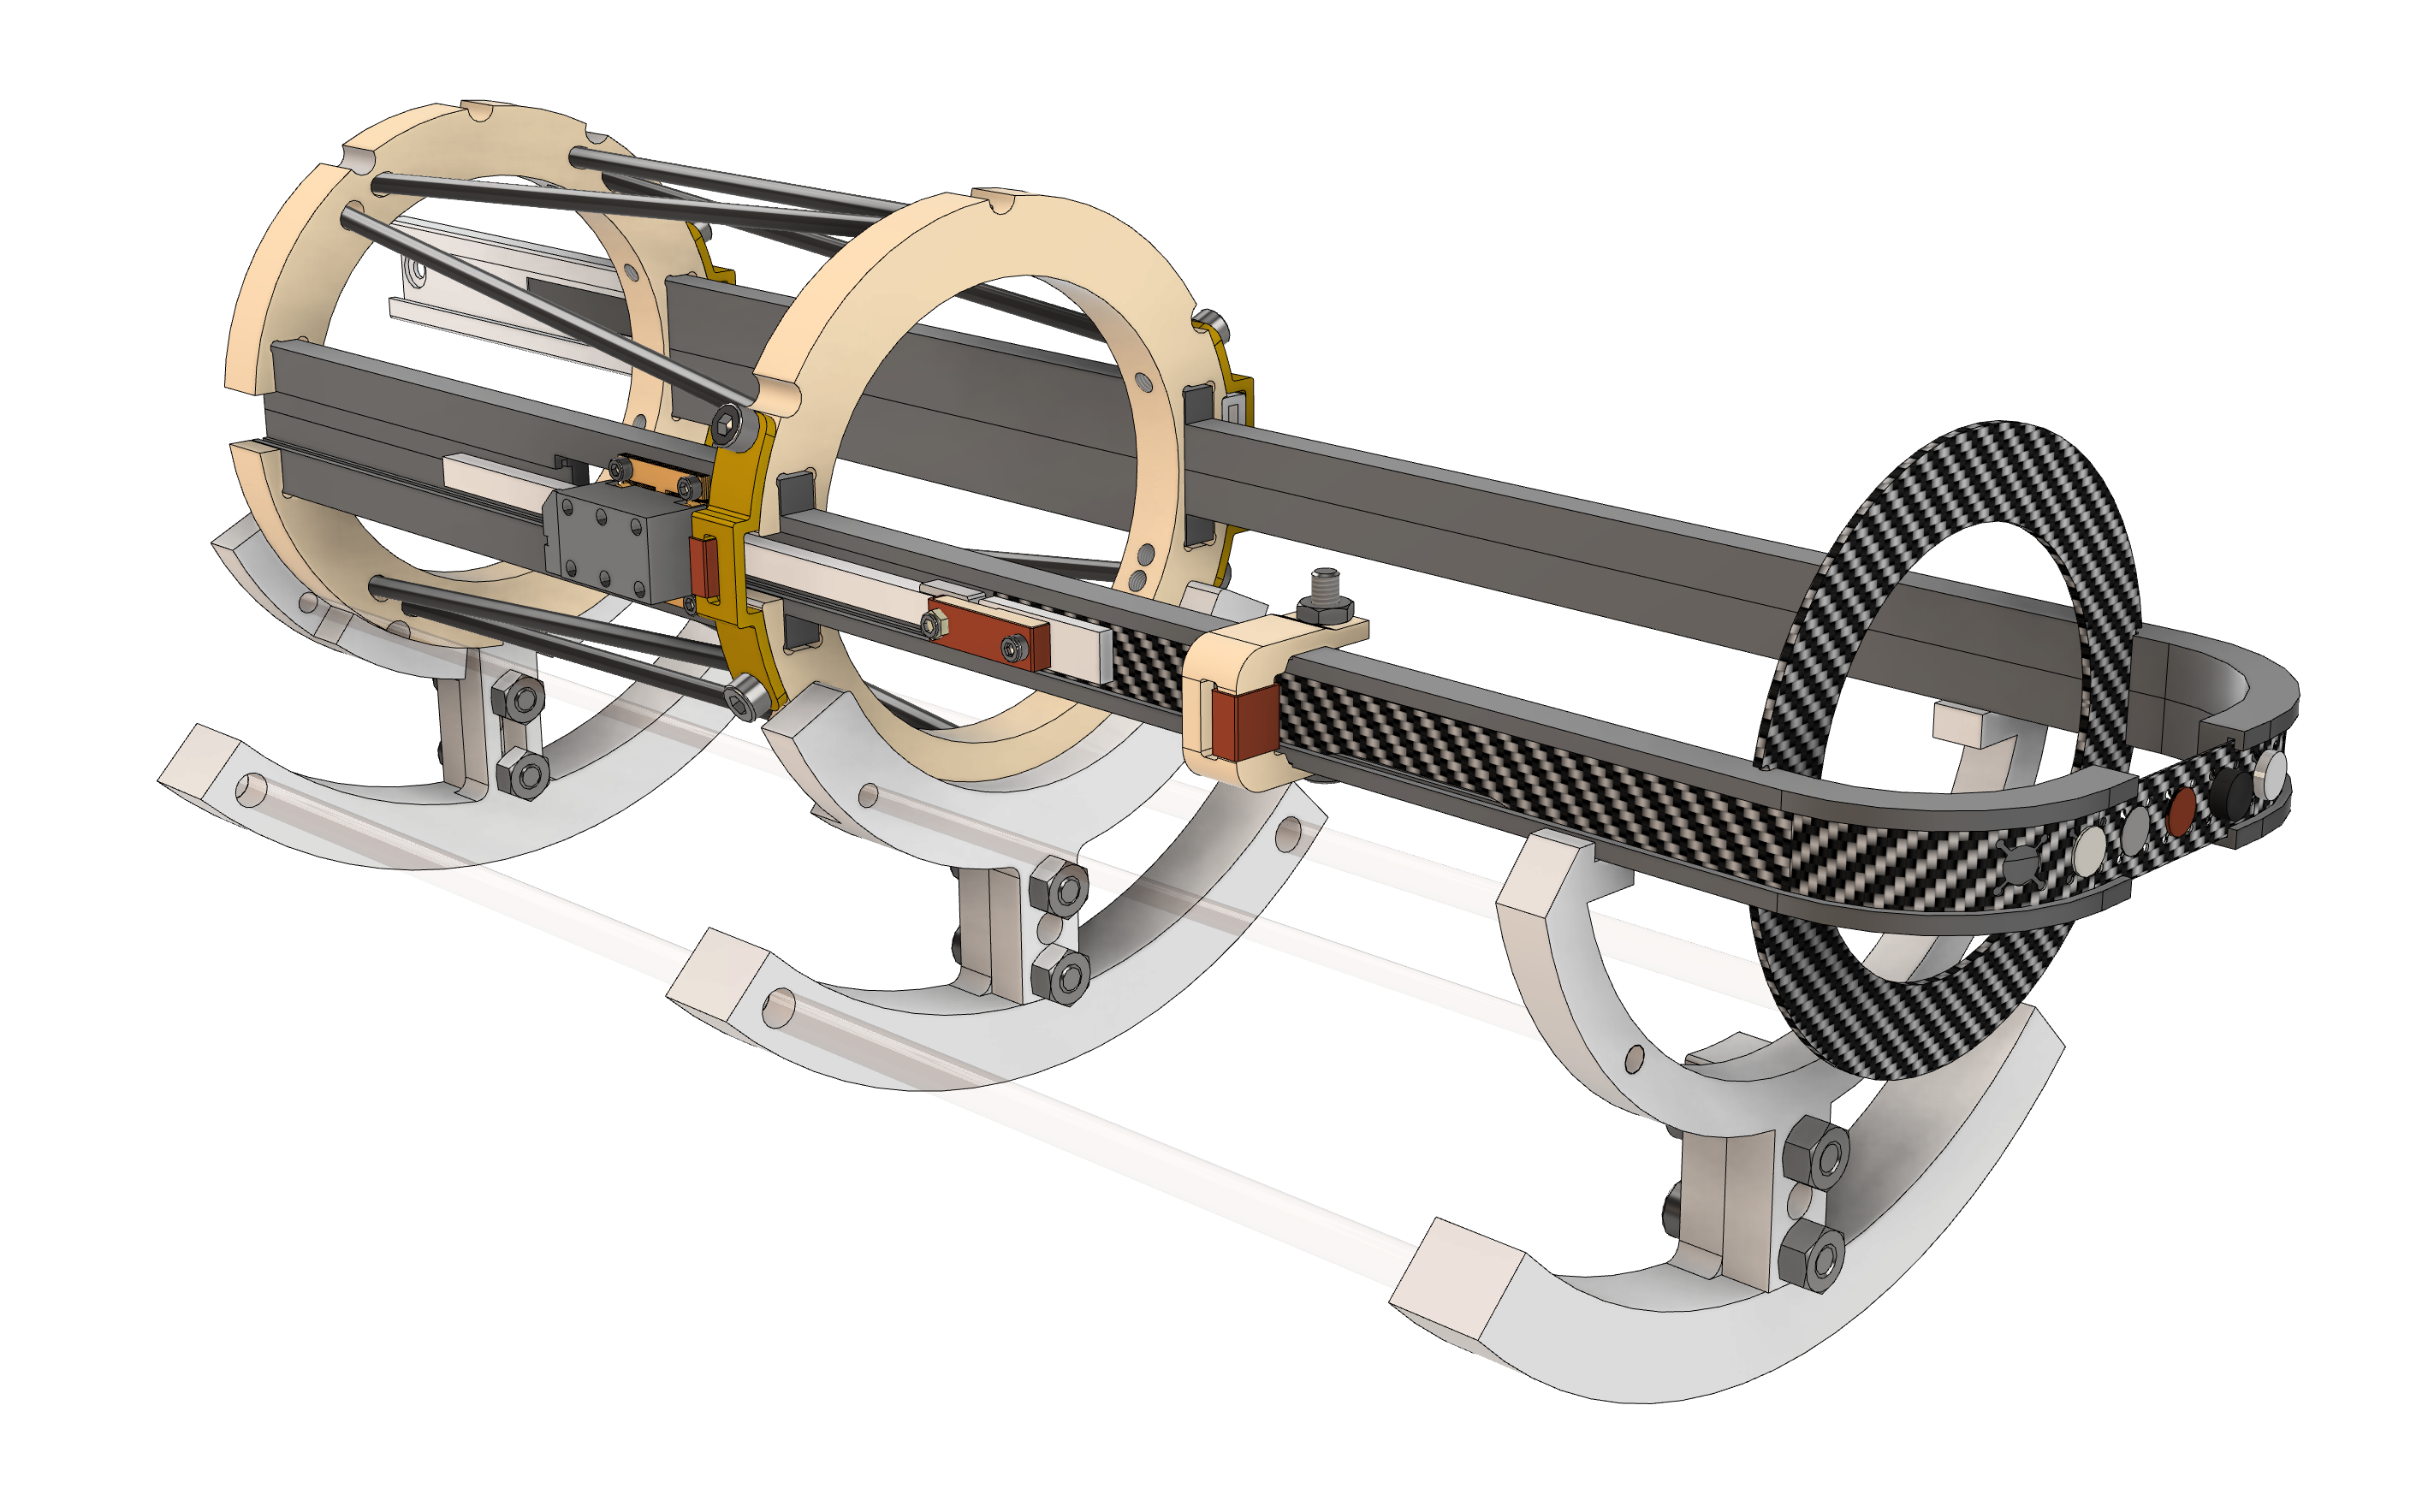
\includegraphics[width=0.5\textwidth]{21double_target.png}}
    %         }
    %
    %         \scriptsize{\textit{
    %             RG-F target CAD render.
    %         }}
    %     \end{figure}
    % \end{center}
\end{frame}
